\documentclass[MASTER-SPC.tex]{subfiles}
\begin{document}
	% MA4605 Lecture 9A Process Capability
\large
\section{Process Capability}
\begin{itemize}
\item In managing variables the usual aim is not to achieve exactly the same diameter for every piston, the same weight for every tablet, sales figures exactly as forecast, etc but to reduce the variation of products and process parameters around a \textbf{target value}. 
	
\item No adjustment of a process is called for as long as there has been no identified change in its accuracy or precision. This means that, in controlling a process, it is necessary to establish first that it is in statistical control, and then to compare it’s centering and spread with the specified target value and specification tolerance.
	
\item We have seen previously that, if a process is not in statistical control, special causes of variation may be identified with the aid of \textbf{\textit{control charts}}. 
	
\item Only when all the special causes have been accounted for, or
	eliminated, can process capability be sensibly assessed. The variation due to common causes may then be examined and the ``\textit{natural specification}" compared with any imposed specification or tolerance zone.
\item The relationship between process variability and tolerances may be formalized by consideration of the standard deviation, $\sigma$, of the process. 
	
	\item In order to manufacture within the specification, the distance between the \textbf{upper specification limit} (USL) or upper tolerance ($+T$) and \textbf{lower specification limit} (LSL) or lower tolerance ($–T$), i.e. ($USL–LSL$) or 2T must be equal to or greater than the width of the base of the process bell, i.e. $6\sigma$.
\end{itemize}

	

	
	\begin{figure}[h!]
		\centering
		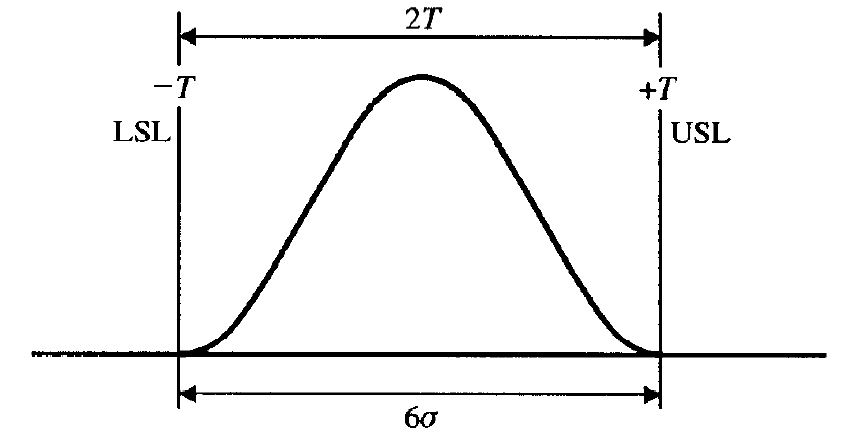
\includegraphics[width=0.8\linewidth]{proccapindices/image1}
	\end{figure}
	
\noindent	The relationship between $USL–LSL$ (i.e. 2T) and $6\sigma$ gives rise
	to three levels of precision of the process (Figure below):
	
	\begin{itemize}
		
		\item[(a)] \textbf{High Relative Precision}, where the tolerance band is very much greater
		than $6\sigma$ ($2T > > 6\sigma$) 
		
		\item[(b)] \textbf{Medium Relative Precision}, where the tolerance band is just greater than
		$6\sigma$ ($2T > 6\sigma$) 
		
		\item[(c)]\textbf{Low Relative Precision}, where the tolerance band is less than
		$6\sigma$ ($2T < 6\sigma$)
	\end{itemize}
\newpage
	\begin{figure}[h!]
		\centering
		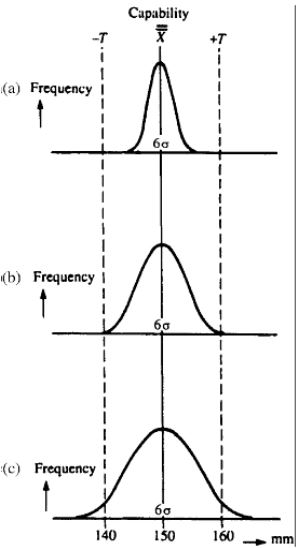
\includegraphics[width=0.60\linewidth]{proccapindices/image1b}
	\end{figure}
	
	\newpage
	\subsection{Process Capability Indices}
\begin{itemize}
\item A process capability index is a measure relating the actual performance of a process to its specified performance, where processes are considered to be a combination of the plant or equipment, the method itself, the people, the materials and the environment. 
\item 	These indices assumes process output is approximately normally distributed.
\item 	
	The absolute minimum requirement is that three process standard deviations each side of the process mean are contained within the specification limits. 
	\item This means that approximately 99.7 per cent of output will be within the tolerances. A more stringent requirement is often stipulated to ensure that produce of the correct quality is consistently obtained over the long term.
	
\item 	When a process is under statistical control (i.e. only random or common
	causes of variation are present), a process capability index may be calculated. 
\item Process capability indices are simply a means of indicating the variability of a process relative to the product specification tolerance.
\end{itemize}	
\newpage


	
	\subsubsection*{C$_p$ index}
\begin{itemize}
\item	In order to manufacture within a specification, the difference between the
	USL and the LSL must be less than the total process variation.
	
\item A comparison of $6\sigma$ with (USL–LSL) or 2T gives an obvious process capability index, known as the $C_p$ of the process:
	
	
	\[\hat{C}_p = \frac{USL - LSL} {6 \hat{\sigma}}\]	
\item This estimates what the process is capable of producing if the process mean were to be centered between the specification limits. 
	Clearly, any value of $C_p$ below 1 means that the process variation is greater than the specified tolerance band so the process is incapable. 
	
\item For increasing values of $C_p$ the process becomes increasingly capable. The $C_p$ index makes no comment about the centring of the process, it is a simple comparison of total variation with tolerances.
\end{itemize}	

\newpage	
	\subsubsection*{$C_{pk}$ index}
\begin{itemize}
\item It is possible to envisage a relatively wide tolerance band with a relatively
	small process variation, but in which a significant proportion of the process output lies outside the tolerance band (Figure below). 
	
	\begin{figure}[h!]
		\centering
		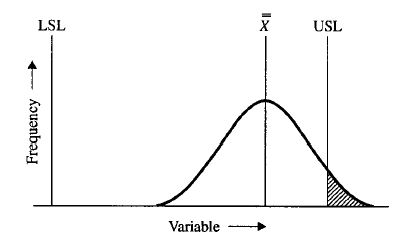
\includegraphics[width=0.7\linewidth]{proccapindices/image3}
	\end{figure}
	
\item This does not invalidate the use of Cp as an index to measure the ‘potential capability’ of a process when centred, but suggests the need for another index which takes account of both the process variation and the centring. Such an index is the $C_{pk}$, which is widely accepted as a means of communicating process capability.
	
	\begin{figure}[h!]
		\centering
		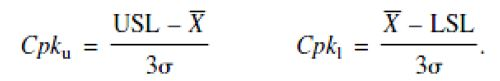
\includegraphics[width=0.7\linewidth]{proccapindices/image4}
	\end{figure}
	
\item 	For upper and lower specification limits, there are two $C_{pk}$ values,
	$C_{pku}$ and $C_{pkl}$. These relate the difference between the process mean and the upper and the lower specification limits respectively, to $3\sigma$ (half the total process variation).
	
\item	The overall process $C_{pk}$ is the lower value of $C_{pku}$ and $C_{pkl}$. A $C_{pk}$ of 1 or less means that the process variation and its centring is such that at least one of the tolerance limits will be exceeded and the process is incapable. As in the case of Cp, increasing values of $C_{pk}$ correspond to increasing capability. 
	
\item	It may be possible to increase the $C_{pk}$ value by centring the process so that its mean value and the mid-specification or target, coincide. A comparison of the Cp and the $C_{pk}$ will show zero difference if the process is centred on the target value.
	
	\begin{figure}[h!]
		\centering
		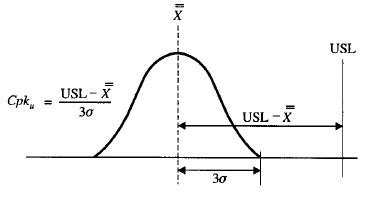
\includegraphics[width=0.7\linewidth]{proccapindices/image5}
	\end{figure}
	
\item	The $C_{pk}$ can be used when there is only one specification limit, upper or lower – a one-sided specification. This occurs quite frequently and the Cp index cannot be used in this situation.
\end{itemize}
\newpage

					\subsection*{Example 1}
					
					\begin{figure}[h!]
						\centering
						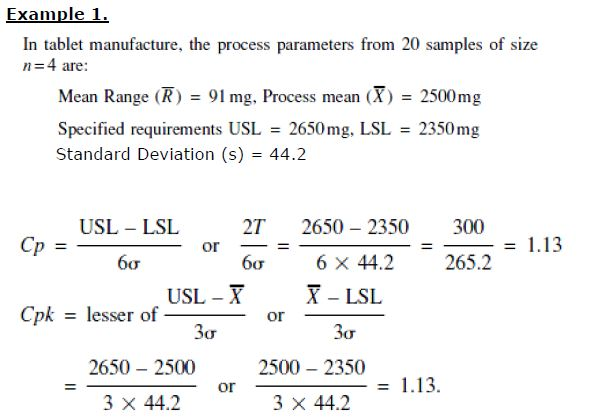
\includegraphics[width=1\linewidth]{proccapindices/Example1}
					\end{figure}
					
					%	Standard Deviation (s) = 44.2
\newpage					
					\subsection*{Example 2}
					
					\begin{figure}[h!]
						\centering
						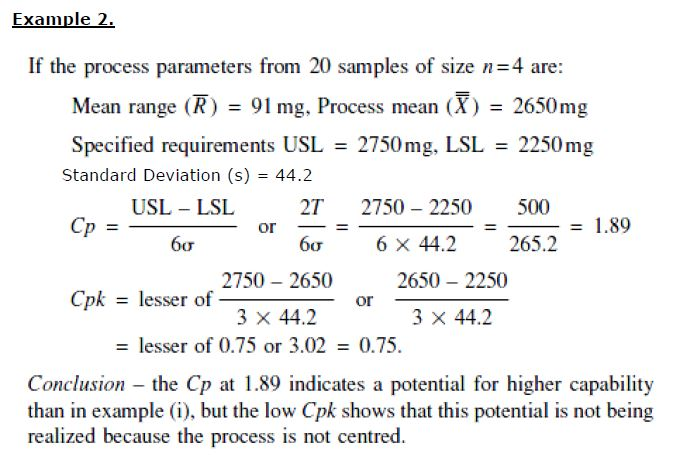
\includegraphics[width=1\linewidth]{proccapindices/Example2}
					\end{figure}
					
					%	Standard Deviation (s) = 44.2
%========================================================== %					
{
	\normalsize
					
\noindent It is important to emphasize that in the calculation of all process capability indices, no matter how precise they may appear, the results are only ever approximations – we never actually know anything, progress lies in obtaining successively closer approximations to the truth. In the case of the process capability this is true because:
					\begin{itemize}
						\item	there is always some variation due to sampling;
						\item	no process is ever fully in statistical control;
						\item	no output exactly follows the normal distribution or indeed any other standard distribution.
					\end{itemize}
					
				
					Interpreting process capability indices without knowledge of the source of the data on which they are based can give rise to serious misinterpretation.
}
\newpage
					
					\subsection*{Interpreting capability indices - IMPORTANT}
					In the calculation of process capability indices so far, we have derived the
					standard deviation, $\sigma$, and recognized that this estimates the short-term variations within the process. This short term is the period over which the process remains relatively stable, but we know that processes do not remain stable for all time and so we need to allow within the specified tolerance limits for:
					
					\begin{itemize}
						\item	some movement of the mean;
						\item	the detection of changes of the mean;
						\item	possible changes in the scatter (range);
						\item	the detection of changes in the scatter;
						\item	the possible complications of non-normal distributions.
					\end{itemize}
					Taking these into account, the following values of the $C_{pk}$ index represent the given level of confidence in the process capability:
					
					\begin{itemize}
						\item	$C_{pk} < 1$ A situation in which the production system is \textbf{not capable} and there will inevitably be non-conforming output from the process.
						
						\item	$C_{pk} = 1$ A situation in which the production system is not really capable, since any change within the process will result in some undetected non-conforming output.
						
						\item	$C_{pk} = 1.33$ A still far from acceptable situation since non-conformance is not likely to be detected by the process control charts.
						
						\item	$C_{pk} = 1.5$ Not yet satisfactory since non-conforming output will occur and the chances of detecting it are still not good enough.
						
						\item	$C_{pk} = 1.67$ Promising, non-conforming output will occur but there is a very good chance that it will be detected.
						
						\item	$C_{pk} = 2$ High level of confidence in the production system, provided that control charts are in regular use.
						
					\end{itemize}
\newpage
					\subsection*{The  $C_{pm}$ Index}
\begin{itemize}
\item	Another Index $C_{pm}$ incorporates the target when calculating the standard deviation. The standard error, denoted $\hat{\sigma}_{Cpm}$ compares each observation to a reference value. \item However, instead of comparing the data to the mean, the data is compared to the target. These differences are squared. Thus any observation that is different from the target observation will increase the $\hat{\sigma}_{Cpm}$  standard deviation.
\item As this difference increases, so does the Cpm. And as this index becomes larger, the $C_{pm}$ gets smaller. 
	
\item If the difference between the data and the target is small, so too is the sigma. And as this sigma gets smaller, the Cpm index becomes larger. The higher the $C_{pm}$ index, the better the process.
	
\item In the following charts the process is the same, but as the process becomes more centred, the $C_{pm}$ gets better.
	\begin{figure}[h!]
		\centering
		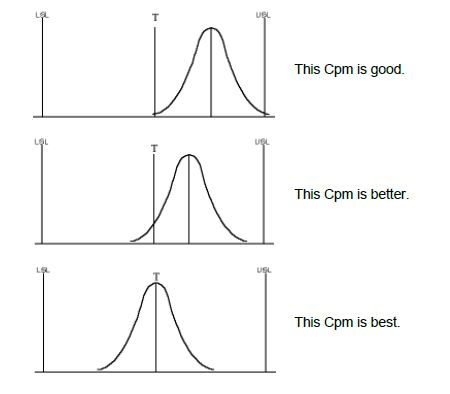
\includegraphics[width=0.7\linewidth]{proccapindices/image6}
	\end{figure}
\end{itemize}
\newpage				
			
			
\noindent  In these 3 charts, the process stays centred about the target, but as the variation is reduced, the Cpm gets better.
			\begin{figure}[h!]
				\centering
				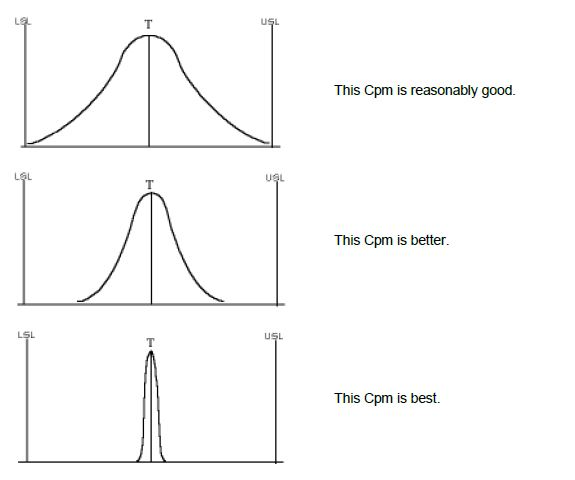
\includegraphics[width=0.8\linewidth]{proccapindices/image7}
			\end{figure}
			
			\begin{figure}[h!]
				\centering
				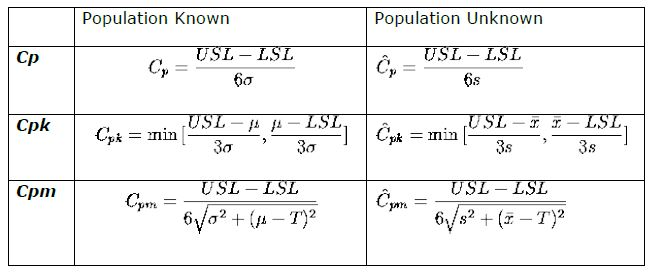
\includegraphics[width=0.8\linewidth]{proccapindices/formulas}
			\end{figure}
			
			\newpage
			\subsection{Worked Example with R}
			
			Data set used – diameter (piston rings data set)
			
			\texttt{R} code used previously, reminding ourselves about the data set.
			
			%data(pistonrings)
			%attach(pistonrings)
			%dim(pistonrings)
			%diameter <- qcc.groups(diameter, sample)
			%obj <- qcc(diameter[1:25,], type="xbar", newdata=diameter[26:40,])
			\begin{figure}[h!]
				\centering
				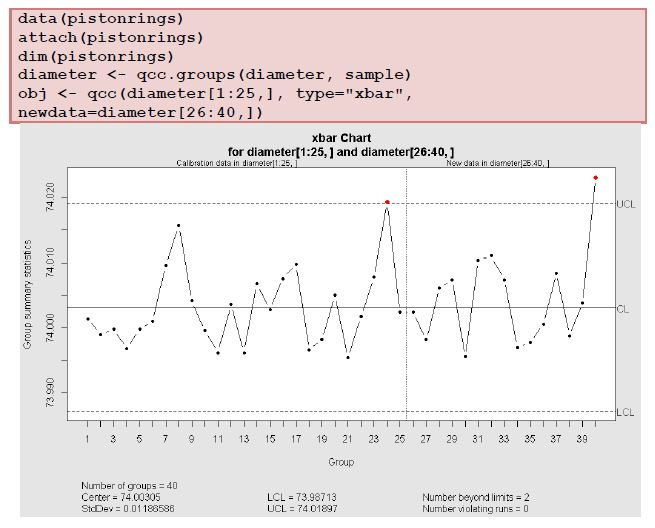
\includegraphics[width=1.1\linewidth]{proccapindices/pistonrings}
			\end{figure}
			
			\newpage
			\subsection{Implementation of Process Capability Analysis}
			Indices and Confidence intervals for those indices.
			
			
\begin{figure}[h!]
\centering
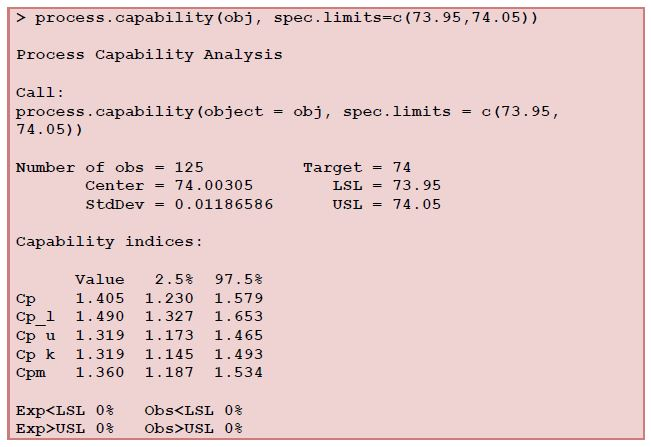
\includegraphics[width=1.1\linewidth]{proccapindices/qccoutput}
\end{figure}
			
			
			\begin{figure}[h!]
\centering
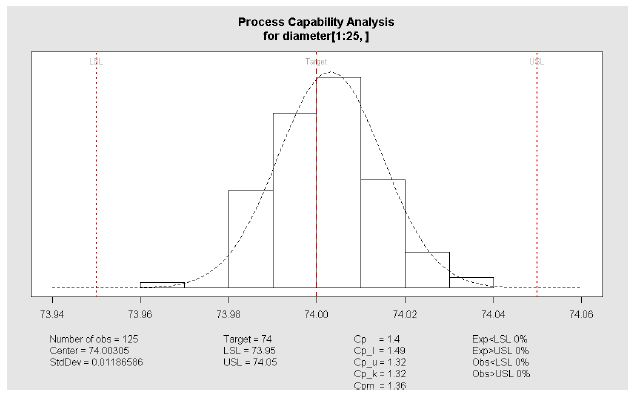
\includegraphics[width=1.1\linewidth]{proccapindices/qcchistogram}
\end{figure}

\end{document}			